\chapter{Учёт эффектов в решении задач смазочного слоя с рельефом поверхности}

\section{Нелинейность}
Безразмерное уравнение Рейнольдса~\eqref{eq:reynolds_nondim}
в зоне полного заполнения смазочного слоя линейно по давлению:
коэффициент~$\bar{h}^{\,3}$ зависит только от геометрии
и не содержит неизвестных. При наличии микроструктур
поверхности линейность по $p$ сохраняется, однако
вычислительная сложность задачи существенно возрастает~\cite{miraskari2018a,miraskari2018b}.
Во-первых, локальные перепады зазора в ячейках микрорельефа
создают резкий контраст коэффициентов: кубическая
зависимость~$h^3$ усиливает разницу между глубокими и мелкими
участками зазора, что ухудшает обусловленность дискретной
системы и замедляет сходимость итерационных решателей
(раздел~3.3). Во-вторых, кавитация в зонах расходящегося
зазора порождает негладкие ограничения~-- переключение между
зонами полного заполнения и кавитации, совместное определение
давления~$p$ и степени заполнения~$\vartheta$ через условия
комплементарности~\eqref{eq:jfo_complementarity}. В-третьих,
при определённых условиях плотность смазки зависит от искомого
давления ($\rho = \rho(p)$), что вносит дополнительную, но уже
гладкую нелинейность. Ниже каждый из перечисленных эффектов
рассматривается отдельно.

\textit{Кавитация как источник негладкой нелинейности.}
Физическая природа кавитации и массосохраняющая постановка JFO
подробно описаны в подразделах~2.3.1-2.3.2. Здесь существенно
то, что постановка JFO~-- это задача с условиями
комплементарности~\eqref{eq:jfo_complementarity}: в каждом узле
либо $p > p_{\mathrm{cav}}$ и $\vartheta = 1$, либо
$p = p_{\mathrm{cav}}$ и $\vartheta < 1$, причём граница между
зонами заранее неизвестна. Вместо единой линейной системы
возникает задача с неравенствами, которая решается итеративно
методом активного множества~-- внешний цикл обновляет
классификацию узлов и пересчитывает~$\vartheta$, а внутренний
цикл решает линейную подсистему для давления при
фиксированном~$\vartheta$ (глава~3, раздел~3.5). Такая
двухуровневая итерационная структура требует согласования
критериев остановки обоих уровней.

При гладком зазоре кавитация, как правило, формирует одну
связную область, положение которой стабилизируется за несколько
внешних итераций. Микроструктуры поверхности принципиально
усложняют картину: каждый элемент микрорельефа создаёт
локальный перепад зазора с зоной разрежения на расходящемся
участке. В результате кавитационная область может формироваться
не в виде одной связной зоны, а в виде множества
фрагментированных «островков», привязанных к отдельным ячейкам
микрорельефа. Активное множество узлов
с~$p = p_{\mathrm{cav}}$ становится разрозненным, его
конфигурация чувствительна к разрешению сетки и к критериям
остановки внешних итераций. Ошибка в определении границы
кавитации даже на один узел изменяет баланс потоков в соседних
ячейках, поэтому требуется достаточное разрешение сетки для
описания каждого элемента микрорельефа (не менее нескольких
узлов на ячейку) и ужесточение критериев сходимости внешнего
цикла по сравнению с задачей для гладкого зазора.

\textit{Роль параметра $\Lambda$ и анизотропия задачи.}
Параметр
$\Lambda = L_1/L_2$~\eqref{eq:nondim_Lambda} определяет
соотношение вкладов продольного ($s_1$) и поперечного ($s_2$)
членов в уравнении~\eqref{eq:reynolds_nondim}:
при $\Lambda \ll 1$ вклад второго члена мал и задача
приближается к одномерной по~$s_1$, при $\Lambda \gtrsim 1$
существенно возрастает роль поперечного растекания по~$s_2$
(коэффициент перед соответствующим членом
равен $\Lambda^2$). Для задач с микроструктурами
значение~$\Lambda$ определяет, насколько локальные эффекты
микрорельефа «размываются» потоком в поперечном направлении.
При большом~$\Lambda$ поперечное растекание сглаживает
возмущения давления от отдельных ячеек; при малом~$\Lambda$
эти возмущения концентрируются вдоль~$s_1$ и оказывают более
сильное влияние на результирующее поле давления и границы
кавитации.

Конкретные значения~$\Lambda$ для трёх постановок монографии
следуют из масштабов таблицы~\ref{tab:nondim_scales}.
Для радиального подшипника $L_1 = R$ (окружной масштаб),
$L_2 = L$ (длина подшипника), и значения $\Lambda = R/L$
соответствуют умеренной или сильной анизотропии в зависимости
от геометрии. Для упорного подшипника $L_1 = R$,
$L_2 = R_{\mathrm{out}} - R_{\mathrm{in}}$
и $\Lambda = R/(R_{\mathrm{out}} - R_{\mathrm{in}})$, как
правило, порядка единицы, т.\,е.\ задача квази-изотропна.
Для возвратно-поступательного подшипника $L_1 = L$ (длина
цилиндра), $L_2 = R$ и $\Lambda = L/R$ может быть значительно
больше единицы; это означает усиление вклада поперечного члена
(по $s_2 = R\theta$) в безразмерном
уравнении~\eqref{eq:reynolds_nondim} и повышенные требования
к разрешению по поперечному направлению.

С вычислительной точки зрения анизотропия задачи требует
согласования шагов сетки по~$s_1$ и~$s_2$. При больших
значениях $\Lambda$ вклад производных по~$s_2$ усиливается
коэффициентом~$\Lambda^2$, и недостаточное разрешение
по «слабому» направлению может приводить
к дискретизационным ошибкам, доминирующим в оценке сходимости
и искажающим вычисленные границы кавитационных зон. Разумная
стратегия~-- выбирать отношение
$\Delta s_1/\Delta s_2$ порядка~$\Lambda$, чтобы
безразмерные шаги сетки были сопоставимы.

\textit{Изменение плотности: гладкая нелинейность
$\rho = \rho(p)$.}
В задачах глав~5-7 смазка предполагается несжимаемой
жидкостью, $\rho = \mathrm{const}$, и плотность не входит
в число неизвестных. Вместе с тем существуют ситуации, когда
это допущение неприемлемо: газовая смазка, большие перепады
давления в высоконагруженных узлах, двухфазные режимы
со значительным изменением массового содержания фаз в области
кавитации. Для полноты постановки здесь приводится обобщение
уравнения JFO~\eqref{eq:jfo_conservation} на случай переменной
плотности в размерной форме:
\begin{equation}
  \frac{\partial (\rho\,\vartheta\,h)}{\partial t}
  + \nabla\cdot\!\left(
      -\frac{\rho\,h^3}{12\mu}\,\nabla p
      + \frac{\rho\,\vartheta\,h}{2}\,\mathbf{U}
    \right) = 0,
  \label{eq:jfo_rho_general}
\end{equation}
где плотность~$\rho = \rho(p)$ входит как в член накопления,
так и в напорный и переносной потоки. В отличие от
комплементарности JFO, зависимость~$\rho(p)$ является гладкой
(задаётся уравнением состояния конкретной среды), поэтому результирующая нелинейность также гладкая
и устраняется итерациями Пикара с релаксацией: на каждой
итерации $\rho$ пересчитывается по полю давления предыдущего
шага, после чего решается обновлённая система. Такой подход
совместим с двухуровневой структурой алгоритма JFO
(раздел~3.5) и не требует изменения внутреннего
решателя~-- достаточно обновлять коэффициенты системы перед
очередной внешней итерацией. Следует подчеркнуть, что
в расчётах глав~5-7 данной монографии
$\rho = \mathrm{const}$
и обобщение~\eqref{eq:jfo_rho_general} не используется;
раздел описывает его для полноты постановки.

\textit{Термовязкость и внешние итерации.}
Гладкая нелинейность возникает и при учёте термовязкостных
эффектов: если вязкость зависит от температуры
($\mu = \mu(T)$), а температура в свою очередь определяется
скоростью диссипации в зазоре, то уравнение Рейнольдса
оказывается связано с уравнением энергии. В этом случае задача
теряет линейность по $p$: при фиксированном поле $T$ (а значит,
$\mu = \mu(T)$) уравнение по-прежнему линейно по давлению,
однако $T$ зависит от градиентов давления и скорости, что
требует итерационного согласования. Типичная стратегия~--
внешний цикл Пикара (fixed-point): на каждой итерации сначала
решается уравнение Рейнольдса при фиксированном поле вязкости,
затем из полученного поля скоростей пересчитывается температура
и вязкость, и цикл повторяется до выхода на согласованное
решение. Сходимость внешнего цикла, как правило, линейная;
число итераций составляет 5--20 в зависимости от интенсивности
тепловых эффектов. В изотермической постановке, принятой
в прикладных главах настоящей монографии, внешний цикл
не требуется: уравнение Рейнольдса решается как линейная
задача при фиксированной $\mu = \mu_0 = \mathrm{const}$.

Подводя итог, наиболее принципиальная нелинейность при
моделировании смазочного слоя с микроструктурами~-- кавитация
в постановке JFO, порождающая задачу с условиями
комплементарности и фрагментированным активным множеством.
Параметр~$\Lambda$ характеризует анизотропию уравнения
Рейнольдса и режим растекания, определяя степень влияния
локальных эффектов микрорельефа на общую картину давления
и конфигурацию кавитационных зон. Зависимость $\rho(p)$
представляет собой опциональное обобщение, применяемое при
наличии физических предпосылок; в расчётах глав~5-7
монографии смазка принимается несжимаемой~\cite{jang2002,rebufa2017}.


\FloatBarrier
\section{Температура}
В разделе~4.1 было показано, что основные нелинейности при
моделировании смазочного слоя с микроструктурами связаны
с кавитацией (негладкая нелинейность постановки JFO)
и, при необходимости, с зависимостью плотности от
давления (гладкая нелинейность $\rho(p)$). Температура
вводит ещё одну гладкую нелинейность~-- через зависимость
динамической вязкости от температуры $\mu = \mu(T)$:
при фиксированном поле температур уравнение
Рейнольдса~\eqref{eq:reynolds_full} остаётся линейным
по давлению, однако вязкость в его коэффициентах сама
зависит от неизвестного поля~$T$, определяемого балансом
генерации и отвода теплоты. Изменение вязкости
непосредственно влияет на распределение давления, несущую
способность, утечки, потери на трение и положение границ
кавитации. Для задач с микроструктурами температурные
эффекты приобретают дополнительное значение: локальные
перепады толщины зазора усиливают градиенты скорости сдвига
и, как следствие, вязкостную диссипацию, что может приводить
к формированию областей с существенно повышенной
температурой в зонах микрорельефа. Стратегия монографии
состоит в том, что расчёты глав~5--7 выполняются
в изотермическом приближении ($T = T_0$, $\mu = \mathrm{const}$);
настоящий раздел формулирует постановку термовязкостного
(THD) расширения, применимую в случаях, когда тепловые
эффекты существенны.

\textit{Источники и отвод тепла в смазочном слое.}
Основным источником теплоты в тонком смазочном слое является
вязкая диссипация~-- необратимое преобразование кинетической
энергии сдвигового течения в теплоту. Для оценки порядка
величины достаточно рассмотреть чисто куэттовский профиль
скорости между двумя поверхностями: удельная мощность
диссипации в пересчёте на единицу площади~$q^{+}$ пропорциональна $\mu(T)\,U^2/h$, где
$U$~-- характерная скорость поверхности, $h$~-- толщина
зазора. Поскольку $q^{+}$ обратно пропорционален~$h$,
в зонах минимального зазора (в том числе у краёв ячеек
микрорельефа) диссипация резко возрастает. Отвод теплоты
из слоя осуществляется тремя каналами: во-первых,
теплопроводностью через стенки~-- от смазки к валу
и вкладышу; во-вторых, конвективным переносом теплоты
потоком самой смазки от входной области к выходной;
в-третьих, теплоотдачей от наружных поверхностей подшипника
в окружающую среду. Соотношение этих каналов определяется
конкретной конструкцией и режимом работы; в рамках
настоящего раздела для полноты постановки рассматриваются
все три механизма. Общая схема теплового баланса
представлена на рисунке~\ref{fig:heat_balance}.

\begin{figure}[!ht]
\centering
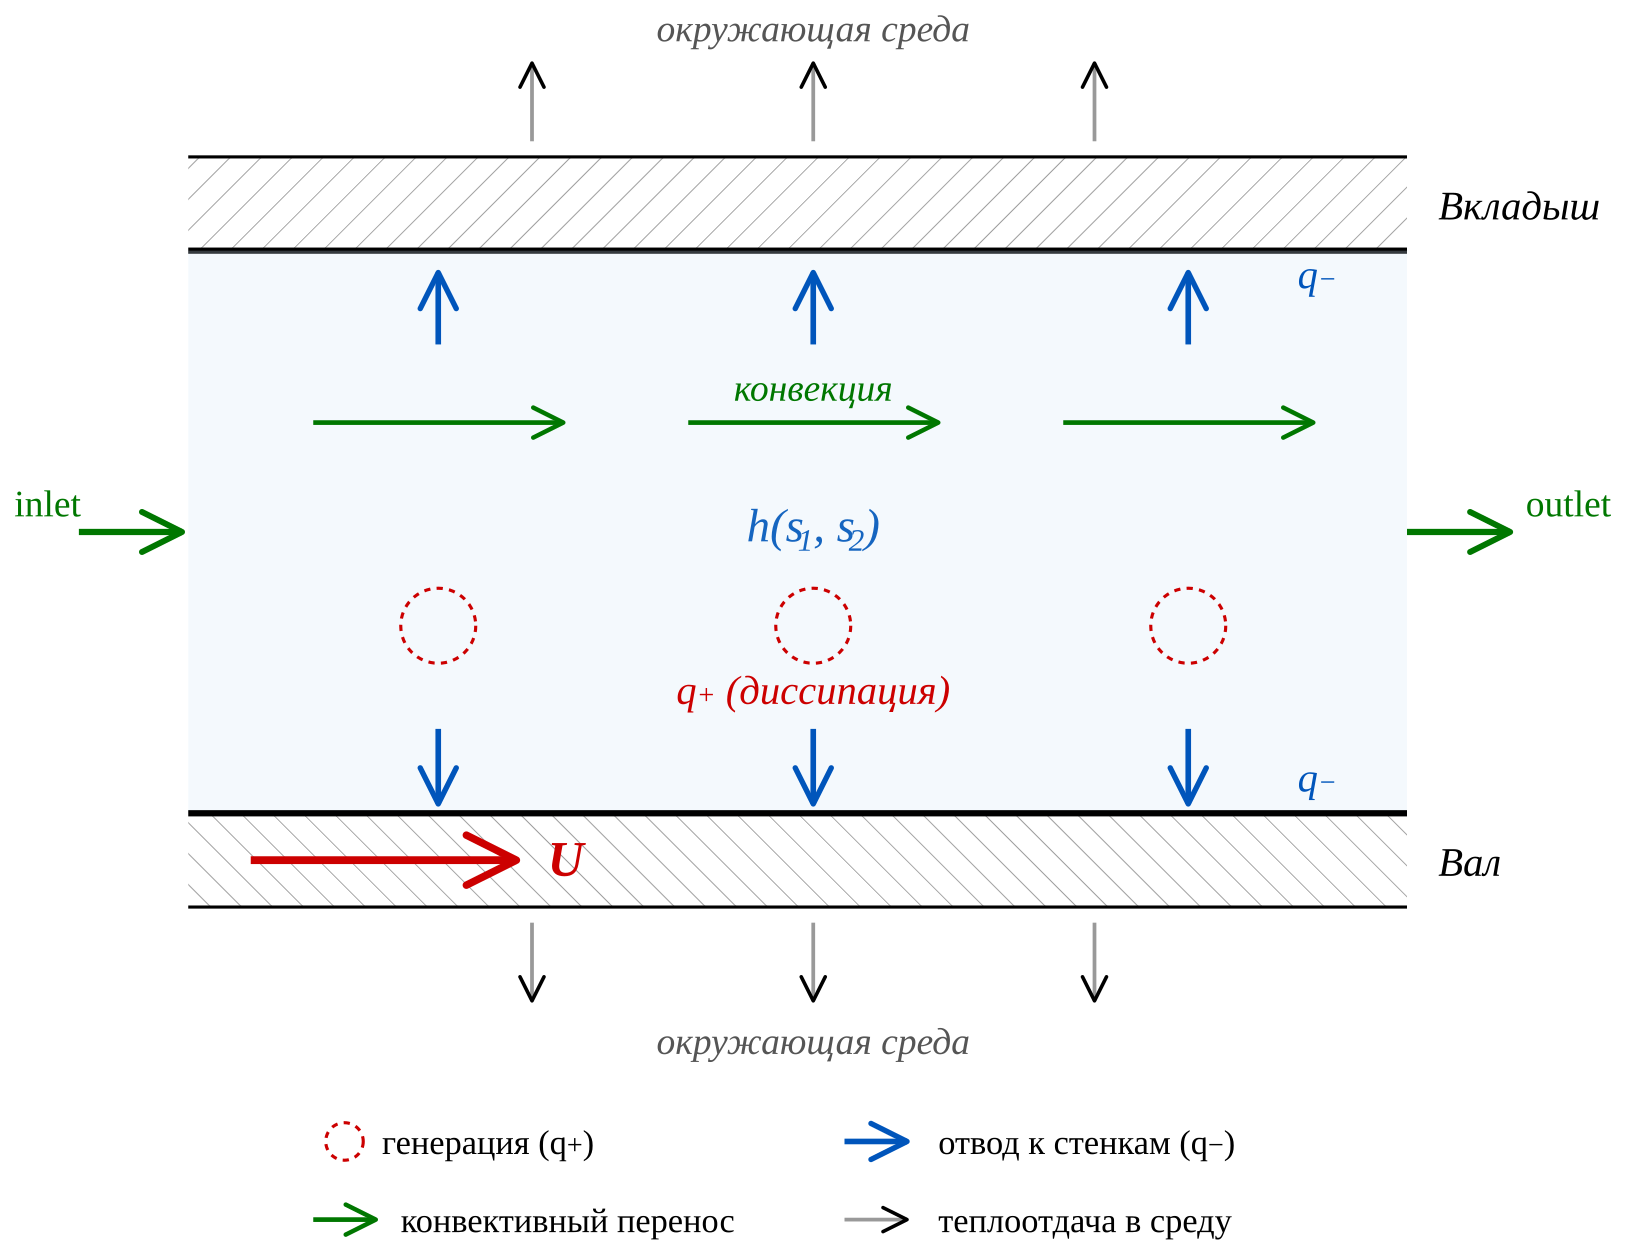
\includegraphics[width=\textwidth,height=0.9\textheight,keepaspectratio]{figures/ch04/fig_4_1.png}
\caption{Источники и каналы отвода теплоты в смазочном слое}
\label{fig:heat_balance}
\end{figure}

\FloatBarrier

\textit{Уровни учёта температуры.}
В зависимости от требуемой точности и вычислительных
ресурсов можно выделить три уровня учёта температуры,
представляющих собой «лестницу сложности» модели.

Первый уровень~-- изотермическое приближение ($T = T_0$,
$\mu = \mu_0 = \mathrm{const}$): температурное поле
не рассчитывается, вязкость принимается постоянной.
Это наиболее простая и распространённая постановка,
используемая в расчётах глав~5--7 настоящей монографии.

Второй уровень~-- приближение эффективной температуры:
сначала решается уравнение Рейнольдса (или задача JFO)
с текущим значением вязкости, затем по полученному полю
давления и скоростей оценивается суммарная диссипация,
вычисляется эффективная температура~$T_{\mathrm{eff}}$
(например, из интегрального теплового баланса), после чего
вязкость обновляется как $\mu(T_{\mathrm{eff}})$
и процедура повторяется до сходимости. Уравнение энергии
в явном виде не решается, что существенно упрощает
реализацию, однако снижает точность при выраженной
неоднородности температурного поля.

Третий уровень~-- термогидродинамика (THD): совместное
решение уравнения Рейнольдса (или задачи JFO) и уравнения
энергии для поля~$T(s_1, s_2, t)$ с учётом зависимости
$\mu(T)$. Этот подход обеспечивает наибольшую точность,
но требует значительных вычислительных затрат, поскольку
на каждой итерации необходимо решать дополнительную краевую
задачу для температуры. Далее в разделе формулируется именно
постановка THD.

\textit{Зависимость вязкости от температуры.}
Для количественного описания влияния температуры
на вязкость необходима аналитическая зависимость $\mu(T)$.
Наиболее употребительным в расчётах тонкоплёночных течений
является экспоненциальный закон:
\begin{equation}
  \mu(T) = \mu_0 \exp\!\bigl(-\beta\,(T - T_0)\bigr),
  \label{eq:viscosity_exp}
\end{equation}
\begin{conditions}
$\mu_0 = \mu(T_0)$ -- вязкость при референсной температуре~$T_0$;\\
$\beta$ -- температурный коэффициент вязкости, $\beta > 0$, K$^{-1}$.
\end{conditions}
При умеренных перепадах температуры (порядка десятков кельвинов)
экспоненциальный закон~\eqref{eq:viscosity_exp} даёт хорошее
приближение и удобен аналитически: производная
$\partial\mu/\partial T = -\beta\,\mu$ линейна по~$\mu$,
что упрощает линеаризацию при итерационном решении.

Для масел в широком диапазоне температур более точным
является трёхпараметрический закон Фогеля:
\begin{equation}
  \mu(T) = A \exp\!\left(\frac{B}{T - C}\right),
  \label{eq:viscosity_vogel}
\end{equation}
\begin{conditions}
$A$, $B$, $C$ -- эмпирические параметры, определяемые
аппроксимацией паспортных данных смазочного масла;\\
$T$ -- абсолютная температура, К.
\end{conditions}
Закон Фогеля~\eqref{eq:viscosity_vogel} лучше описывает
нелинейность кривой $\mu(T)$ при больших температурных
перепадах, однако его параметризация требует экспериментальных
данных. В обоих случаях зависимость $\mu(T)$ является гладкой
и монотонно убывающей~-- повышение температуры приводит
к уменьшению вязкости, что, в свою очередь, снижает несущую
способность и увеличивает утечки, создавая обратную связь
между тепловым и гидродинамическим полями (рисунок~\ref{fig:viscosity_temp}).

\begin{figure}[!ht]
\centering
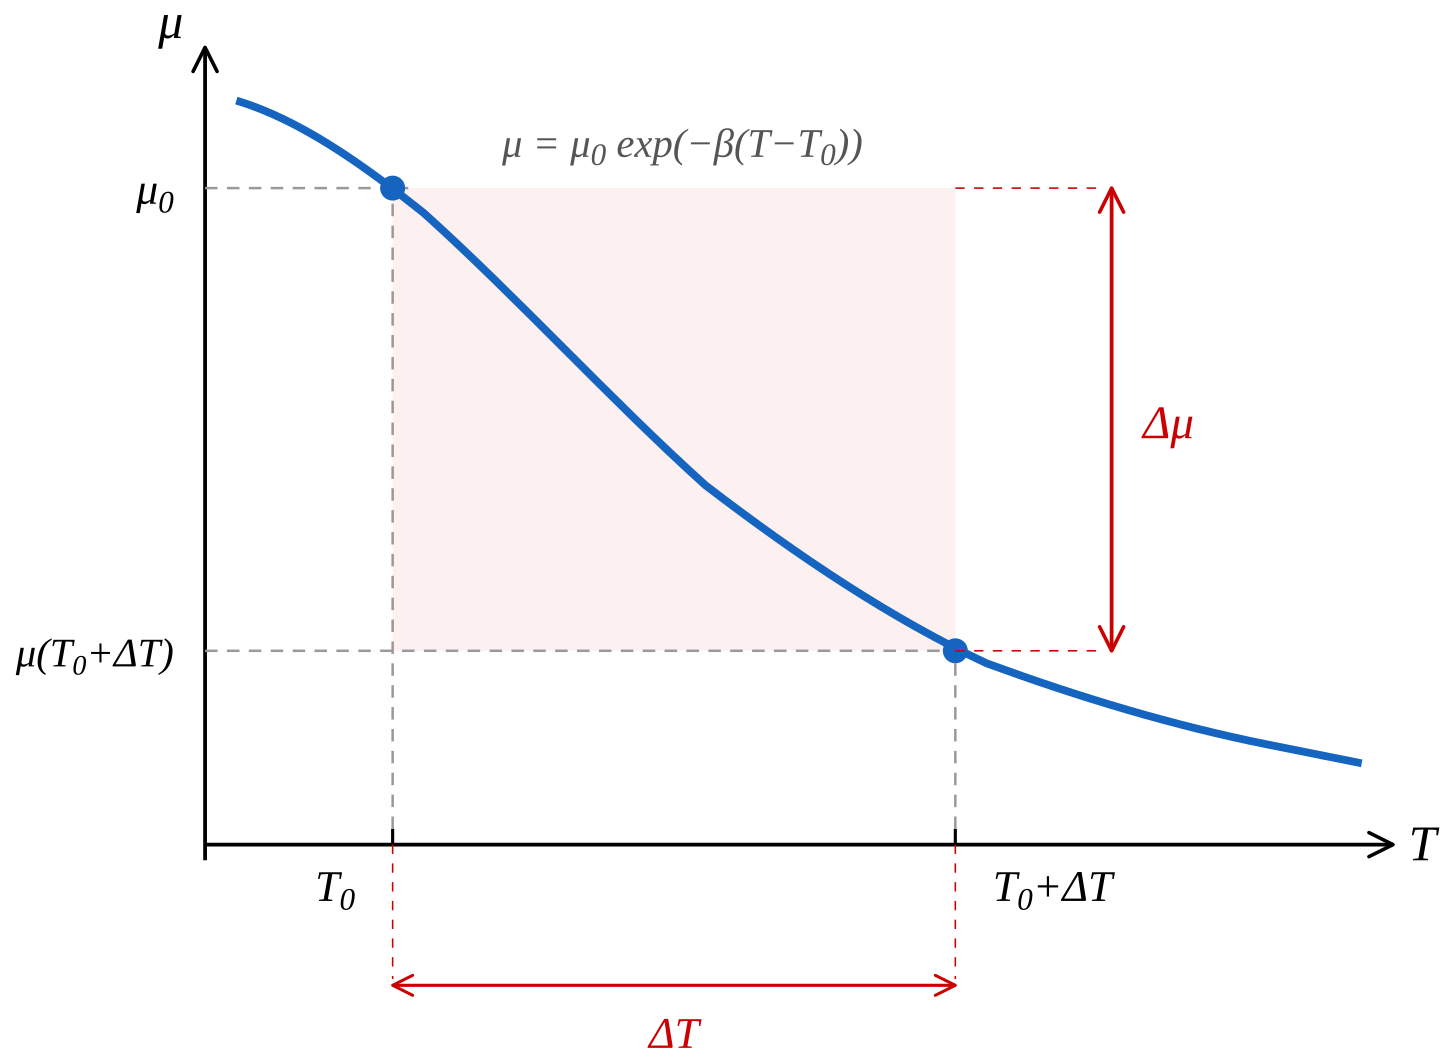
\includegraphics[width=\textwidth,height=0.9\textheight,keepaspectratio]{figures/ch04/fig_4_2.png}
\caption{Типовая температурная зависимость вязкости смазки}
\label{fig:viscosity_temp}
\end{figure}

\FloatBarrier

\textit{Уравнение энергии для смазочного слоя.}
Для описания температурного поля на третьем уровне учёта
(THD) необходимо уравнение энергии. Аналогично тому, как
в разделе~4.1 обобщение JFO с переменной плотностью
записывалось в размерной форме, уравнение энергии здесь
также приводится в размерных переменных. Используется
двумерная плёночная постановка, усреднённая по толщине
зазора:
\begin{equation}
  \rho\,c_p\,h\,\frac{\partial T}{\partial t}
  + \rho\,c_p\,h\,(\mathbf{u}_{\parallel} \cdot \nabla T)
  = \nabla\cdot(k_{\parallel}\,h\,\nabla T)
    + q^{+} - q^{-},
  \label{eq:energy_film}
\end{equation}
\begin{conditions}
$\mathbf{u}_{\parallel}$ -- средняя по толщине скорость
в плоскости $(s_1,\,s_2)$;\\
$c_p$ -- удельная теплоёмкость смазки при постоянном
давлении;\\
$k_{\parallel}$ -- эффективная теплопроводность смазки
в плоскости плёнки;\\
$q^{+}$ -- удельная мощность тепловыделения на единицу площади опорной поверхности, обусловленная вязкой диссипацией; оценка порядка: $q^{+} \sim \mu(T)\,U^2/h$;\\
$q^{-}$ -- удельная мощность теплоотвода на единицу площади к стенкам (валу и вкладышу).
\end{conditions}
Левая часть уравнения~\eqref{eq:energy_film} описывает
нестационарное накопление теплоты и её конвективный перенос
потоком смазки; правая часть~-- диффузию теплоты в плоскости
плёнки, генерацию за счёт диссипации и отвод к ограничивающим
поверхностям.

Средние по толщине скорости $\mathbf{u}_{\parallel}$ вычисляются по стандартным выражениям для тонкого слоя (суперпозиция куэттовского и пуазейлевского профилей) на основе полей $p$, $h$ и $\mu$, полученных на текущей итерации решателя.

\textit{Упрощённая конвективная модель как частный случай.}
В ряде практических постановок общее уравнение
энергии~\eqref{eq:energy_film} допускает существенное упрощение. Ниже приведён вариант для радиальной постановки, где $s_1 = \varphi$~-- окружная координата, $s_2 = Z = z/L$~-- безразмерная осевая координата, $H = h/c_0$~-- безразмерная толщина зазора, $c_0$~-- характерный радиальный зазор подшипника, $P$~-- безразмерное давление в соответствии с безразмеризацией подраздела~2.1.3.
Если принять стационарное приближение ($\partial T/\partial t = 0$),
пренебречь диффузией теплоты в плоскости плёнки
($\nabla\cdot(k_{\parallel}\,h\,\nabla T) \approx 0$) и считать,
что конвективный перенос теплоты осуществляется преимущественно
вдоль окружного направления~$\varphi$,
уравнение~\eqref{eq:energy_film} сводится к конвективной форме. В данной редуцированной постановке теплоотвод к стенкам явно не учитывается (формально $q^{-} \approx 0$); тепловой баланс замыкается конвективным переносом и условием частичного перемешивания на входе~\eqref{eq:bc_partial_mix}:
\begin{equation}
  \mathrm{Pe}\cdot H\,\frac{\partial T}{\partial\varphi}
  = Q_{\mathrm{total}}\cdot\Delta T_{\mathrm{ref}},
  \label{eq:energy_convective}
\end{equation}
где $\mathrm{Pe} = \rho\,c_p\,U\,c_0/k$~-- число Пекле,
характеризующее соотношение конвективного и кондуктивного переноса
теплоты ($k$~-- теплопроводность смазки); $H = h/c_0$~-- безразмерная толщина зазора;
$\Delta T_{\mathrm{ref}}$~-- опорный температурный перепад, используемый при безразмеризации уравнения энергии.
Уравнение~\eqref{eq:energy_convective} является рабочей формой
тепловой модели, реализованной в расчётном модуле.
Уравнение~\eqref{eq:energy_convective} представляет собой ОДУ по~$\varphi$ и решается численным интегрированием по окружности совместно с условием~\eqref{eq:bc_partial_mix}.

Безразмерный источник теплоты~$Q_{\mathrm{total}}$ объединяет вклады
вязкого сдвига (доминирующий) и напорного течения
(пропорциональный~$H^3$):
\begin{equation}
  Q_{\mathrm{total}} = \frac{1}{H}
  + \gamma\,H^3\!\left[
      \left(\frac{\partial P}{\partial\varphi}\right)^{\!2}
      + \left(\frac{D}{L}\right)^{\!2}
        \left(\frac{\partial P}{\partial Z}\right)^{\!2}
    \right],
  \label{eq:Q_total}
\end{equation}
где $P$~-- безразмерное давление; $D$,~$L$~-- диаметр и длина
подшипника; $\gamma$~-- коэффициент, определяемый выбранными
масштабами безразмеризации (в реализованной модели $\gamma = 0{,}1$).
Первое слагаемое~$1/H$ отражает сдвиговую диссипацию Куэтта, второй
член~-- дополнительный вклад пуазейлевской компоненты течения от
градиента давления.

Граничное условие на входе задаётся в виде частичного перемешивания
свежей смазки с нагретой после полного оборота:
\begin{equation}
  T\big|_{\varphi=0}
  = \tfrac{1}{2}\,T_{\mathrm{inlet}}
  + \tfrac{1}{2}\,T\big|_{\varphi=2\pi},
  \label{eq:bc_partial_mix}
\end{equation}
где $T_{\mathrm{inlet}}$~-- температура подаваемой свежей смазки.
Условие~\eqref{eq:bc_partial_mix} моделирует ситуацию, при которой
масло на входе в зазор представляет собой равную смесь свежего масла
и масла, прошедшего полный оборот; в результате эффективная
температура на входе оказывается выше~$T_{\mathrm{inlet}}$, что
соответствует реальному тепловому балансу в подшипнике с непрерывной
циркуляцией смазки.

В полной постановке~\eqref{eq:energy_film} теплоотвод к стенкам задаётся явно через~$q^{-}$; ниже приведены два типовых варианта. При известных температурах стенок используются условия первого рода:
\[
  T_{\mathrm{wall},1} = \mathrm{const}, \qquad
  T_{\mathrm{wall},2} = \mathrm{const},
\]
и~$q^{-}$ определяется из решения поперечного профиля
температуры. Альтернативный, более гибкий подход~-- задание
эффективного конвективного теплоотвода:
\[
  q^{-} = \alpha_1\,(T - T_{\mathrm{wall},1})
         + \alpha_2\,(T - T_{\mathrm{wall},2}),
\]
где $\alpha_1$,~$\alpha_2$~-- коэффициенты теплоотдачи,
определяемые условиями конкретной задачи (геометрией,
теплопроводностью материалов, режимом течения).

Граничные условия для уравнения~\eqref{eq:energy_film}
в плоскости~$(s_1, s_2)$ задаются следующим образом:
на входной границе смазочного слоя температура задана
($T = T_{\mathrm{in}}$), на выходной границе принимается
условие свободного выхода ($\partial T/\partial n = 0$).

\textit{Алгоритм термовязкостного итерационного цикла.}
Совместное решение уравнения Рейнольдса (или задачи JFO)
и уравнения энергии~\eqref{eq:energy_film} с зависимостью
$\mu(T)$ осуществляется итерационно. Структура алгоритма
совместима с двухуровневой схемой решения JFO, описанной
в разделе~3.5: температурный цикл выполняется как
дополнительный внешний уровень, охватывающий циклы
по давлению и кавитации. Последовательность шагов
на каждой итерации~$m$ выглядит следующим образом.
\begin{enumerate}[wide, labelindent=\parindent, nosep]
  \item Задать начальное поле
    $T^{(0)} = T_0$ и вычислить начальную вязкость
    $\mu^{(0)} = \mu(T_0)$.
  \item Решить уравнение Рейнольдса или задачу JFO
    с текущим полем вязкости~$\mu^{(m)}$; получить
    давление~$p^{(m)}$ и поле скоростей.
  \item Решить уравнение энергии~\eqref{eq:energy_film}
    с источником~$q^{+}$, определённым по~$p^{(m)}$
    и~$\mu^{(m)}$; получить обновлённое
    поле~$T^{(m+1)}$.
  \item Применить релаксацию по температуре:
    $T^{(m+1)} \leftarrow (1 - \omega_T)\,T^{(m)}
    + \omega_T\,T^{(m+1)}$,
    где $\omega_T \in (0,\,1]$~-- параметр релаксации;
    после релаксации обновить вязкость:
    $\mu^{(m+1)} = \mu(T^{(m+1)})$ по
    закону~\eqref{eq:viscosity_exp}
    или~\eqref{eq:viscosity_vogel}.
  \item Проверить критерии сходимости; при их выполнении
    остановиться, в противном случае вернуться к шагу~2.
\end{enumerate}

Критерии сходимости формулируются по отклонениям полей
температуры и давления между последовательными итерациями:
\begin{equation}
  \|\,T^{(m+1)} - T^{(m)}\| < \varepsilon_T, \qquad
  \|\,p^{(m+1)} - p^{(m)}\| < \varepsilon_p.
  \label{eq:thd_convergence}
\end{equation}

Параметр релаксации~$\omega_T$ выбирается из условия
устойчивости итераций; при сильной зависимости~$\mu(T)$
(больших значениях~$\beta$ в~\eqref{eq:viscosity_exp})
может потребоваться умеренная подрелаксация
($\omega_T = 0{,}3\text{--}0{,}7$). Важно отметить, что
описанный алгоритм совместим с кэшированием GPU-буферов
(раздел~3.4): при обновлении~$\mu$ на каждой итерации
достаточно пересчитать коэффициенты дискретизации без
переразмещения памяти на устройстве.

\textit{Тепловые эффекты при наличии микроструктур.}
Микроструктуры поверхности существенно модифицируют
тепловую картину смазочного слоя по сравнению с гладким
зазором. Впадины и ячейки микрорельефа создают локальные
зоны с повышенным градиентом скорости сдвига: поскольку
удельная мощность диссипации пропорциональна $\mu\,U^2/h$,
в местах минимального зазора~-- у краёв и на гребнях ячеек~--
источник~$q^{+}$ возрастает резко и нелинейно. При гладком
зазоре диссипация распределена по полю относительно
равномерно; при наличии микротекстур возникают локальные
«горячие пятна», где температура может существенно превышать
среднюю по плёнке (рисунок~\ref{fig:hotspots_texture}).

\begin{figure}[!ht]
\centering
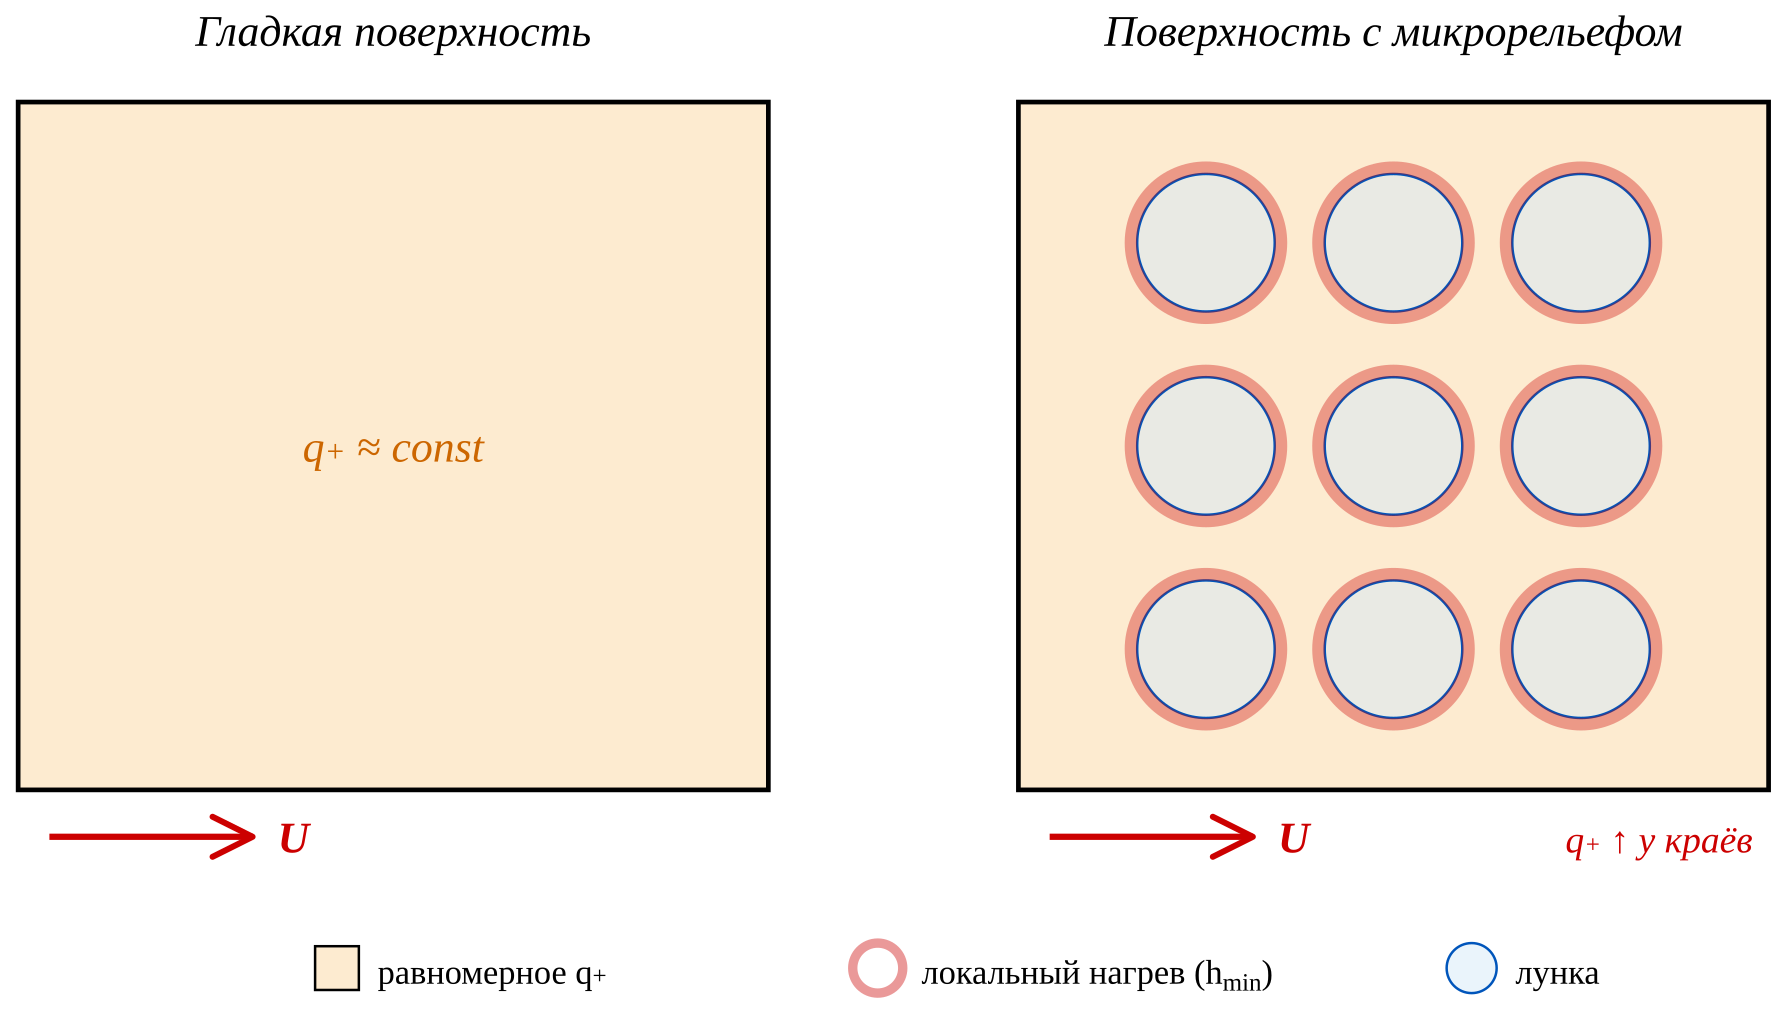
\includegraphics[width=\textwidth,height=0.9\textheight,keepaspectratio]{figures/ch04/fig_4_3.png}
\caption{Локализация диссипации при наличии микротекстур (схема):
  гладкая поверхность (слева) и поверхность с микрорельефом (справа)}
\label{fig:hotspots_texture}
\end{figure}

\FloatBarrier

Это означает, что средняя температура смазочного слоя может
оставаться умеренной, тогда как локальный нагрев в зонах
микрорельефа оказывается значительным и способен повлиять
на несущую способность и границы кавитации. Для корректного
описания таких эффектов необходимо разрешение расчётной
сетки, достаточное для детального представления каждой ячейки
микрорельефа; это требование согласуется с требованиями
по разрешению кавитационных зон, сформулированными
в разделе~4.1. Кавитация (степень заполнения $\vartheta < 1$)
дополнительно модифицирует перенос теплоты в двухфазной
зоне~-- снижение плотности и теплоёмкости газожидкостной
смеси изменяет баланс
уравнения~\eqref{eq:energy_film}; в рамках настоящего
раздела этот эффект детально не раскрывается, однако
представляет собой направление возможного расширения модели.

В расчётах глав~5--7 используется изотермическое
приближение: $T = T_0$, $\mu = \mathrm{const}$. Такой подход
оправдан при умеренных скоростях скольжения и нагрузках, когда
температурный перепад в слое мал и его влияние на вязкость
несущественно. Постановка THD, изложенная
в настоящем разделе, обеспечивает основу для расширения модели
в случаях, когда тепловые эффекты становятся определяющими~--
в частности, при высоких скоростях скольжения, использовании
вязких масел или при глубоких микроструктурах с локально
высокой диссипацией~\cite{kyrkou2020,pierre2004,sun2010,talaighil2015}.


\FloatBarrier
\section{Шероховатость поверхности}
Предметом настоящей монографии являются детерминированные
микроструктуры~-- регулярные элементы заданной геометрии (лунки,
канавки, текстуры), описываемые явным полем добавки~$\Delta h$
в суперпозиции зазора~\eqref{eq:h_superposition} и параметризованные
в подразделе~2.2. Наряду с детерминированным рельефом любая
обработанная поверхность содержит шероховатость~-- случайную
составляющую топографии, возникающую при механической обработке,
полировке или лазерном текстурировании. Шероховатость
характеризуется не явной геометрией, а статистическими параметрами:
среднеарифметическим отклонением профиля~$R_a$,
среднеквадратичным отклонением~$R_q$ и длиной
корреляции~$\lambda_c$. Настоящий раздел устанавливает, при каких
условиях шероховатость существенно влияет на решение задачи
и какие подходы позволяют учесть её при необходимости.

\textit{Критерий значимости шероховатости.}
Определяющим безразмерным параметром является отношение
характерной толщины смазочного слоя~$h_0$ к среднеквадратичной
шероховатости:
\begin{equation}
  \lambda_r = \frac{h_0}{R_q}\,,
  \label{eq:lambda_roughness}
\end{equation}
\begin{conditions}
$h_0$ -- характерная толщина зазора, м;\\
$R_q$ -- комбинированная среднеквадратичная шероховатость
контактирующих поверхностей, м.
\end{conditions}
В задачах с микроструктурами критерием режима служит локальное значение $\lambda_r(s_1, s_2) = h(s_1, s_2)/R_q$; в качестве интегральной оценки режима смазки используют минимальную толщину плёнки~$h_{\min}$, либо характерный минимум~$h_0$.

Параметр~$\lambda_r$ называется числом смазочного слоя
(\textit{film thickness ratio}) и определяет режим взаимодействия
поверхностей. При $\lambda_r \gg 1$ (условно $\lambda_r > 5$)
поверхности надёжно разделены плёнкой смазки, высота
шероховатостей пренебрежимо мала по сравнению с толщиной зазора,
и поле давления определяется макрогеометрией и детерминированным
микрорельефом. При $\lambda_r \approx 1\text{--}3$ высота
микронеровностей становится соизмеримой с толщиной зазора,
шероховатость начинает взаимодействовать с полем давления, и для
адекватного описания потоков требуются модифицированные уравнения.
При $\lambda_r < 1$ реализуется режим граничной смазки
с непосредственным контактом микронеровностей; рейнольдсовская
модель тонкого слоя в этом режиме неприменима.

Для типичных подшипниковых задач с детерминированными
микроструктурами значение~$\lambda_r$ составляет 3--10, что
соответствует режиму гидродинамической смазки. Глубина ячейки
микрорельефа~$h_p = H_p \cdot h_0$ (подраздел~2.2.4,
формула~\eqref{eq:Hp_nondim}) при типичных значениях
$H_p \sim 0{,}1\text{--}1$ существенно превышает амплитуду
шероховатости: $h_p \gg R_q$. Иерархия масштабов~-- базовый
зазор, детерминированная текстура и шероховатость~-- схематически
представлена на рисунке~\ref{fig:roughness_scales}. Это
соотношение масштабов обосновывает допущение о гладкости
поверхностей, принятое в расчётах глав~5--7.

\begin{figure}[!ht]
\centering
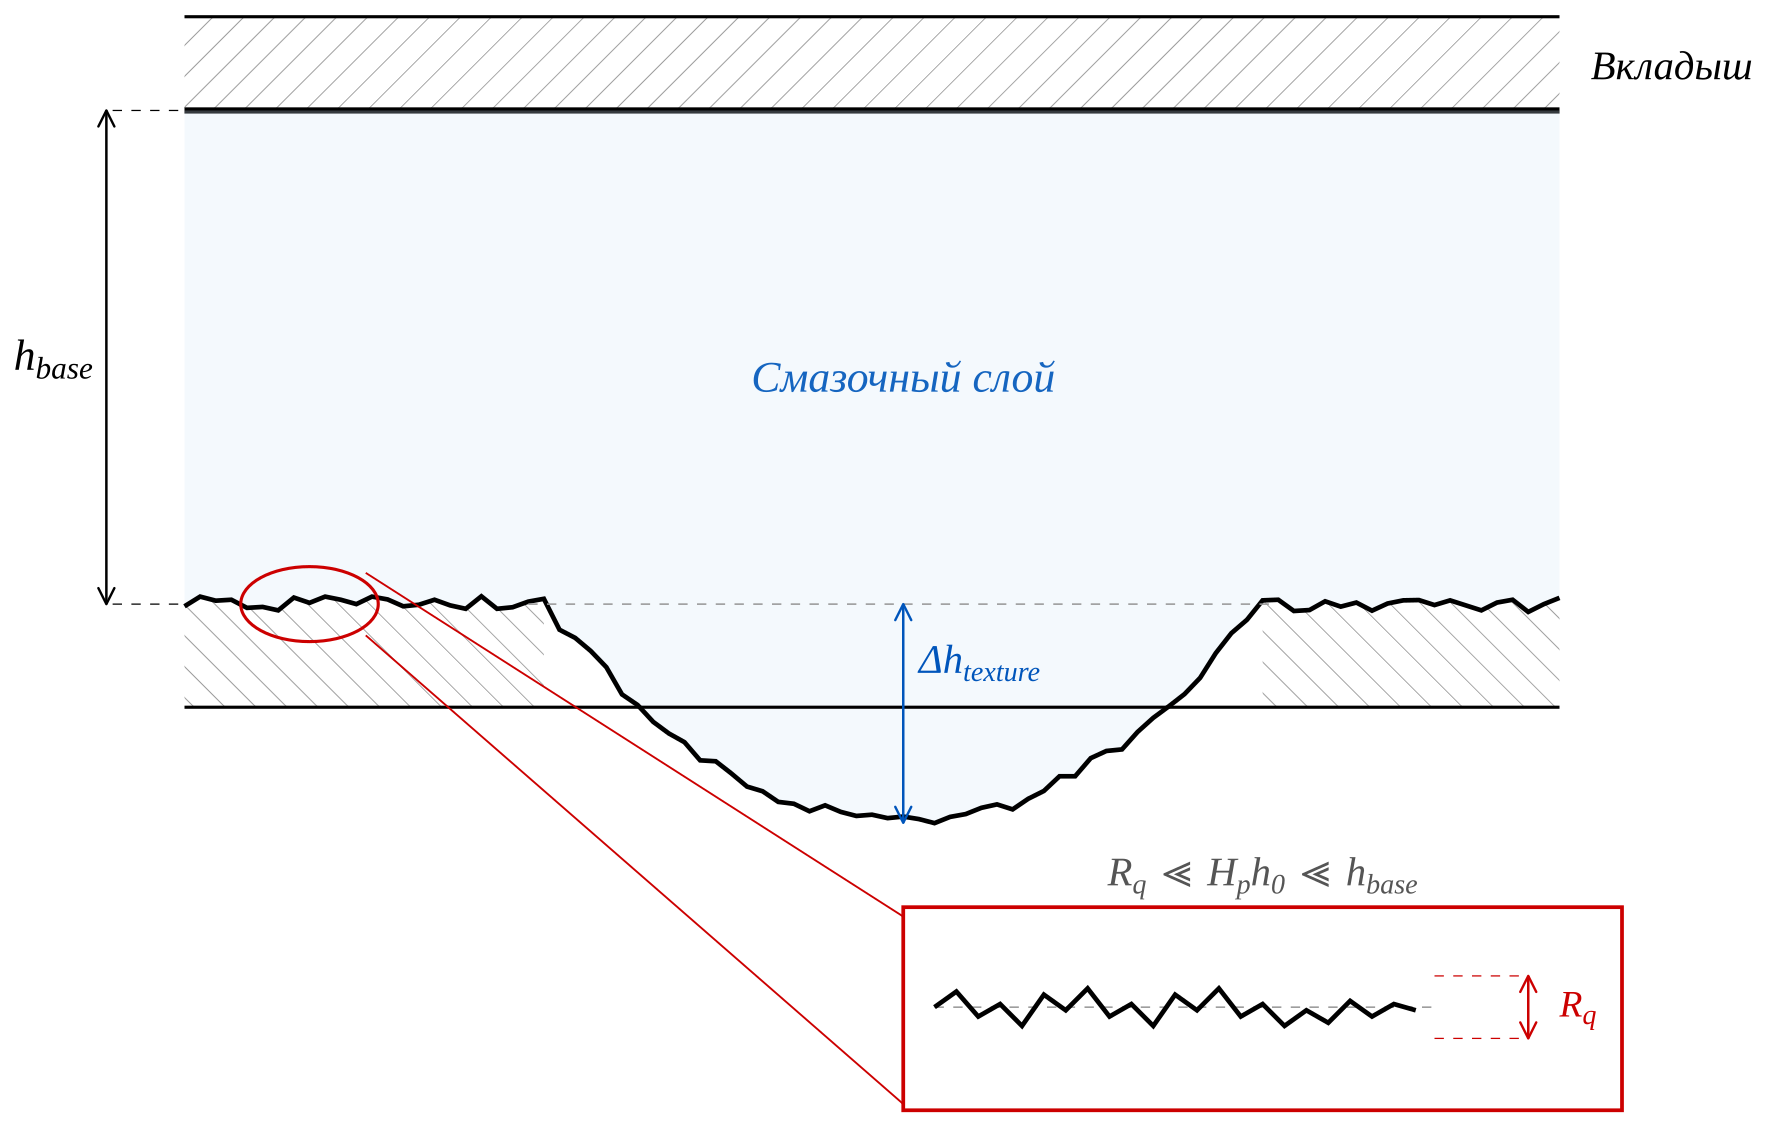
\includegraphics[width=\textwidth,height=0.9\textheight,keepaspectratio]{figures/ch04/fig_4_4.png}
\caption{Иерархия масштабов топографии поверхности:
  базовый зазор, детерминированная микротекстура и шероховатость}
\label{fig:roughness_scales}
\end{figure}

\FloatBarrier

\textit{Подходы к учёту шероховатости в уравнении Рейнольдса.}
В литературе сложились три основных подхода, различающихся
по сложности реализации и области применимости.

Первый подход~-- детерминированный: шероховатость задаётся явным
полем $\Delta h_{\mathrm{rough}}(s_1, s_2)$, полученным по данным
измерений (атомно-силовая микроскопия, контактная профилометрия),
и добавляется в суперпозицию зазора наряду с текстурой:
\[
  h = h_{\mathrm{base}} + \Delta h_{\mathrm{texture}}
    + \Delta h_{\mathrm{rough}}.
\]
Такой подход требует измеренного профиля поверхности
и разрешения расчётной сетки, достаточного для представления
случайного рельефа: шаг сетки должен быть существенно меньше
длины корреляции~$\lambda_c$ (единицы микрометров). Это приводит
к значительному увеличению числа узлов по сравнению с задачей для
гладких поверхностей (глава~3) и обоснованно только в рамках
исследовательских расчётов.

Второй подход~-- стохастический, основанный на осреднении
уравнения Рейнольдса по ансамблю реализаций случайной
шероховатости. Пионерская модель Кристенсена (Christensen, 1969)
и её развитие в работах Патира и Ченга (Patir, Cheng, 1978--1979)
вводят поправочные коэффициенты (\textit{flow factors}), которые
учитывают влияние статистической шероховатости на средние потоки
смазки. Осреднённое уравнение Рейнольдса записывается для
среднего давления~$\bar{p}$ с модифицированными коэффициентами:
\begin{equation}
  \frac{\partial}{\partial s_1}\!\left(\phi_p\,\bar{h}^3\,
  \frac{\partial \bar{p}}{\partial s_1}\right)
  + \Lambda^2\frac{\partial}{\partial s_2}\!\left(\phi_p\,\bar{h}^3\,
  \frac{\partial \bar{p}}{\partial s_2}\right)
  = \phi_s\,\frac{\partial \bar{h}}{\partial s_1}
  + \phi_c\,\sigma_r\,\frac{\partial \phi_s}{\partial s_1}\,,
  \label{eq:reynolds_rough_avg}
\end{equation}
\begin{conditions}
$\bar{h}$ -- номинальная (без случайной составляющей) толщина зазора: $\bar{h} = h_{\mathrm{base}} + \Delta h_{\mathrm{texture}}$ (суперпозиция~\eqref{eq:h_superposition} без~$\Delta h_{\mathrm{rough}}$);\\
$\bar{p}$ -- осреднённое давление;\\
$\phi_p$ -- фактор давления (pressure flow factor),
корректирующий пуазейлевский поток;\\
$\phi_s$ -- фактор сдвига (shear flow factor),
корректирующий куэттовский поток;\\
$\phi_c$ -- контактный фактор;\\
$\sigma_r$ -- суммарная среднеквадратичная шероховатость
контактирующих поверхностей, м ($\sigma_r \equiv R_q$ из~\eqref{eq:lambda_roughness});\\
$\Lambda$ -- отношение масштабов длины
(подраздел~2.1.6).
\end{conditions}
Факторы~$\phi_p$, $\phi_s$ зависят от отношения~$\bar{h}/\sigma_r$
и от ориентации шероховатости (продольная, поперечная,
изотропная). Они вычисляются однократно по статистическим
параметрам поверхности и не требуют разрешения случайного поля
на расчётной сетке, что делает стохастический подход
вычислительно эффективным. Структура
уравнения~\eqref{eq:reynolds_rough_avg} сохраняет форму исходного
уравнения Рейнольдса~\eqref{eq:reynolds_full}, поэтому солверы
и алгоритмы, описанные в главе~3, могут быть адаптированы
с минимальными изменениями. Член с~$\phi_c$ представляет дополнительную поправку, связанную с контактными эффектами при малых значениях~$\lambda_r$; в чисто гидродинамическом режиме ($\lambda_r > 5$) он мал и может быть опущен.

Третий подход~-- пренебрежение шероховатостью: при $\lambda_r \gg 1$
полагается $\Delta h_{\mathrm{rough}} = 0$, и уравнение Рейнольдса
решается для номинального зазора~\eqref{eq:h_superposition}. Это
допущение принято в расчётах глав~5--7 настоящей монографии.

\textit{Взаимодействие шероховатости с детерминированными
микроструктурами.}
При совместном присутствии детерминированных микроструктур
и случайной шероховатости характерные масштабы могут различаться
на порядки. Глубина ячейки микрорельефа~$h_p = H_p \cdot h_0$
составляет, как правило, единицы микрометров (в зависимости от технологии и назначения подшипника) при характерном размере
ячейки в десятки микрометров; шероховатость полированных
поверхностей характеризуется значениями $R_q \sim 0{,}01\text{--}0{,}1$~мкм
при длине корреляции $\lambda_c \sim 1\text{--}10$~мкм.

Когда $R_q \ll H_p \cdot h_0$~-- типичный случай при хорошо
обработанных поверхностях~-- детерминированные микроструктуры
доминируют в формировании поля давления и потоков, а вклад
шероховатости сводится к слабому стохастическому возмущению,
не влияющему на интегральные характеристики подшипника.

Когда $R_q$ оказывается соизмерима с~$H_p \cdot h_0$, что
возможно при грубой обработке или мелком микрорельефе,
шероховатость модифицирует распределение давления внутри ячеек
текстуры, изменяет локальные кавитационные зоны
(раздел~4.1) и может как усилить, так и ослабить эффективность
текстурирования. В этом режиме результаты, полученные в рамках
модели гладких поверхностей, требуют поправок, и корректное
описание предполагает использование одного из рассмотренных выше
подходов~-- детерминированного или стохастического.

Практический вывод для проектирования состоит в том, что
глубина детерминированных микроструктур~$h_p$ должна существенно
превышать среднеквадратичную шероховатость ($H_p \cdot h_0 \gg R_q$),
чтобы регулярный рельеф не терял функциональности на фоне случайных
микронеровностей. Это условие одновременно обеспечивает
$\lambda_r \gg 1$, при котором пренебрежение шероховатостью
в уравнении Рейнольдса обосновано.

В расчётах глав~5--7 поверхности приняты гладкими:
$\Delta h_{\mathrm{rough}} = 0$. Допущение оправдано при
$\lambda_r \gg 1$ и $H_p \cdot h_0 \gg R_q$, что типично
для прецизионных подшипников с полированными поверхностями.
Стохастический подход с коэффициентами потоков~$\phi_p$,
$\phi_s$~\eqref{eq:reynolds_rough_avg} представляет наиболее
практичный путь расширения модели на случай существенной
шероховатости: он сохраняет структуру дискретизации и не требует
разрешения случайного поля на расчётной сетке.
Детерминированный подход применим при наличии измеренных профилей
поверхности и вычислительных ресурсов для высокого разрешения
сетки, характерного масштаба $\lambda_c$.
При необходимости кавитация учитывается постановкой JFO для осреднённого давления~$\bar{p}$, т.\,е.\ условия комплементарности~\eqref{eq:jfo_complementarity} применяются к уравнению~\eqref{eq:reynolds_rough_avg}~\cite{gu2017,nie2022}.

\textit{Физический смысл коэффициентов потока Патира--Ченга.}
В модели Патира--Ченга~\cite{patir1978} исходное уравнение
Рейнольдса заменяется осреднённым уравнением с коэффициентами
потока $\phi_x$, $\phi_y$ (по давлению) и $\phi_s$ (по сдвигу):
%
\begin{equation}
  \frac{\partial}{\partial x}\!\left[\phi_x\,\bar{h}^3\,
  \frac{\partial \bar{p}}{\partial x}\right]
  + \frac{\partial}{\partial y}\!\left[\phi_y\,\bar{h}^3\,
  \frac{\partial \bar{p}}{\partial y}\right]
  = 6\mu U\,\frac{\partial}{\partial x}\!\left(\bar{h}
  + \phi_s\,\sigma_{\mathrm{eq}}\right).
  \label{eq:patir_cheng}
\end{equation}
%
Коэффициент $\phi_s$ описывает дополнительный перенос смазки
за счёт шероховатости (неоднородности переносного потока),
а $\phi_x$, $\phi_y$ отражают анизотропное сопротивление
шероховатости напорному потоку. Все три коэффициента зависят
от параметра $\lambda_r = \bar{h}/\sigma_{\mathrm{eq}}$
и ориентации шероховатости (изотропная, продольная,
поперечная). При $\lambda_r \gg 1$ все коэффициенты стремятся
к единице и уравнение~\eqref{eq:patir_cheng} вырождается
в классическое уравнение Рейнольдса.
При $\lambda_r < 3$ поправки становятся существенными:
$\phi_x$ и $\phi_y$ снижаются ниже единицы (шероховатость
затрудняет напорное течение), тогда как $\phi_s$ может
превышать единицу или быть меньше в зависимости от ориентации.

\textit{Обоснование допущения о гладких поверхностях.}
Допущение о гладких поверхностях ($\phi_x = \phi_y = 1$,
$\phi_s = 0$) принято в прикладных расчётах настоящей работы.
Его обоснование: параметр
$\lambda_r = h_{\min}/\sigma_{\mathrm{eq}}$ в характерных
режимах составляет $\lambda_r \geq 2$ (смешанный режим),
при котором поправки Патира--Ченга имеют ограниченное влияние
на интегральные характеристики и слабо меняют сравнительный
вывод о преимуществе текстурированного варианта над гладким.
Кроме того, детерминированная текстура (глубина
$H_p = 0{,}2$--$0{,}4$ в единицах зазора) по амплитуде
существенно превосходит стохастическую шероховатость
(характерная высота
$\sigma_{\mathrm{eq}} \ll h_{\min}$), поэтому вклад
случайного микрорельефа в интегральные характеристики
подшипника значительно меньше вклада детерминированных лунок.
Включение модели Патира--Ченга потребовало бы ввода
дополнительных параметров (тип и ориентация шероховатости,
коэффициенты потока), которые выходят за рамки исследуемых
переменных, не изменяя качественных выводов работы.


% \FloatBarrier
% \section{Динамика смазочного слоя}
% % sec_4_4_dynamics.tex — Динамика смазочного слоя

Разделы~4.1--4.3 рассматривали нелинейные эффекты применительно к~стационарному вращению вала при~фиксированном положении его~центра. В~реальных условиях эксплуатации вал совершает малые колебания относительно равновесного положения под~действием дисбаланса, переходных нагрузок и~гидродинамических возмущений. Реакция смазочного слоя на~эти~колебания описывается линеаризованными коэффициентами жёсткости и~демпфирования, которые определяют динамические свойства опорного узла и~устойчивость роторной системы в~целом~\cite{goodwin1997,jang1999,sayed2022,muszynska1988,weissbacher2014}.

\textit{Линеаризация по~малым возмущениям положения вала.}
Равновесное положение центра вала характеризуется координатами~$(x_0,\,y_0)$ или, эквивалентно, эксцентриситетом~$\varepsilon_0$ и~углом нагружения~$\psi_0$. При~малом возмущении центр вала смещается в~положение~$(x_0 + \xi,\; y_0 + \eta)$, где~$|\xi|,\,|\eta| \ll c$.

Безразмерная толщина зазора с~учётом возмущения записывается в~виде
\begin{equation}
  H(\theta,\,t) = H_0(\theta)
    - \bar{\xi}(t)\,\cos\theta
    - \bar{\eta}(t)\,\sin\theta,
  \label{eq:H_perturbed}
\end{equation}
\begin{conditions}
$H_0(\theta) = 1 + \varepsilon_0\cos\theta$ -- равновесный зазор радиального подшипника~\eqref{eq:journal_h};\\
$\bar{\xi} = \xi/c$,\; $\bar{\eta} = \eta/c$ -- безразмерные составляющие возмущения положения центра вала.
\end{conditions}
Давление разлагается по~малому параметру:
\begin{equation}
  P = P_0
    + \bar{\xi}\,P_{\xi}
    + \bar{\eta}\,P_{\eta}
    + \dot{\bar{\xi}}\,P_{\dot\xi}
    + \dot{\bar{\eta}}\,P_{\dot\eta}
    + \ldots
  \label{eq:P_expansion}
\end{equation}
Здесь~$P_0$~-- стационарное давление (главы~5--7); поля~$P_{\xi}$, $P_{\eta}$, $P_{\dot\xi}$, $P_{\dot\eta}$ находятся из~линеаризованных уравнений Рейнольдса с~правыми частями, получаемыми дифференцированием~\eqref{eq:reynolds_nondim} по~соответствующим переменным.

В~постановке JFO~\eqref{eq:jfo_conservation} граница кавитационной области при~возмущении может смещаться. В~первом приближении используется допущение о~фиксированной кавитационной области (\textit{frozen cavitation}): граница~$\partial\Omega_{\mathrm{cav}}$ определяется по~равновесному полю~$P_0$. Альтернативные подходы и~их~сравнение рассматриваются в~главе~8.

\textit{Матрицы жёсткости и~демпфирования смазочного слоя.}
Линеаризация гидродинамической силы приводит к~выражению
\begin{equation}
  \begin{pmatrix} \Delta F_x \\ \Delta F_y \end{pmatrix}
  = -\mathbf{K}
  \begin{pmatrix} \bar\xi \\ \bar\eta \end{pmatrix}
  - \mathbf{C}
  \begin{pmatrix} \dot{\bar\xi} \\ \dot{\bar\eta} \end{pmatrix},
  \label{eq:linearized_force}
\end{equation}
где~компоненты матриц жёсткости~$\mathbf{K}$ и~демпфирования~$\mathbf{C}$ определяются как
\begin{equation}
  K_{ij} = -\frac{\partial F_i}{\partial \bar{q}_j}\bigg|_0, \qquad
  C_{ij} = -\frac{\partial F_i}{\partial \dot{\bar{q}}_j}\bigg|_0,
  \quad i,j \in \{x,\,y\},
  \label{eq:KC_def}
\end{equation}
а~численное вычисление выполняется интегрированием возмущённых давлений по~области смазочного слоя:
\begin{equation}
  K_{xx} = -\iint_\Omega P_{\xi}\,\cos\theta\;d\theta\,dZ, \qquad
  K_{xy} = -\iint_\Omega P_{\eta}\,\cos\theta\;d\theta\,dZ,
  \label{eq:K_integrals}
\end{equation}
аналогично для~$K_{yx}$, $K_{yy}$ и~для~$C_{xx}$, $C_{xy}$, $C_{yx}$, $C_{yy}$ через~$P_{\dot\xi}$, $P_{\dot\eta}$.

Детерминированные микроструктуры изменяют стационарное поле~$P_0$ и~возмущённые поля~$P_{\xi}$, $P_{\eta}$, $P_{\dot\xi}$, $P_{\dot\eta}$, а~следовательно, компоненты~$K_{ij}$ и~$C_{ij}$. Это~является основным каналом влияния текстуры поверхности на~динамические характеристики опорного узла. Матрицы~$\mathbf{K}$ и~$\mathbf{C}$ в~общем случае несимметричны: перекрёстные коэффициенты~$K_{xy} \neq K_{yx}$, $C_{xy} \neq C_{yx}$, что~обусловлено вращательным характером течения смазки и~является принципиальным отличием подшипников скольжения от~упругих опор.

\textit{Критерии устойчивости роторно-подшипниковой системы.}
Уравнение движения ротора массой~$M$ в~двухкоординатной ($2$DOF) модели записывается в~виде
\begin{equation}
  M\,\ddot{\mathbf{q}} + \mathbf{C}\,\dot{\mathbf{q}} + \mathbf{K}\,\mathbf{q} = 0,
  \qquad \mathbf{q} = (\bar\xi,\,\bar\eta)^T.
  \label{eq:rotor_eom}
\end{equation}
Переход к~переменным состояния~$\mathbf{u} = (\mathbf{q},\,\dot{\mathbf{q}})^T$ приводит систему к~стандартной форме
\begin{equation}
  \dot{\mathbf{u}} = \mathbf{A}\,\mathbf{u}, \qquad
  \mathbf{A} =
  \begin{pmatrix}
    \mathbf{0} & \mathbf{I} \\
    -M^{-1}\mathbf{K} & -M^{-1}\mathbf{C}
  \end{pmatrix}.
  \label{eq:state_matrix}
\end{equation}
Система асимптотически устойчива тогда и~только тогда, когда все~собственные значения~$\lambda_k$ матрицы~$\mathbf{A}$ имеют отрицательную вещественную часть: $\mathrm{Re}(\lambda_k) < 0$ для~всех~$k$. Если~хотя~бы~для~одного~$k$ выполняется~$\mathrm{Re}(\lambda_k) > 0$, система неустойчива; граничный случай~$\max_k \mathrm{Re}(\lambda_k) = 0$ соответствует порогу устойчивости (критической скорости).

Формулы для~критических скоростей и~интегральных критериев устойчивости зависят от~конкретной модели ротора (масса, жёсткость вала, гироскопика) и~в~данном разделе не~приводятся; количественный пример применительно к~подшипнику центробежного насоса рассматривается в~главе~8.

Общая схема линеаризованной модели сил смазочного слоя
приведена на рисунке~\ref{fig:linearized_forces}.

\begin{figure}[!ht]
\centering
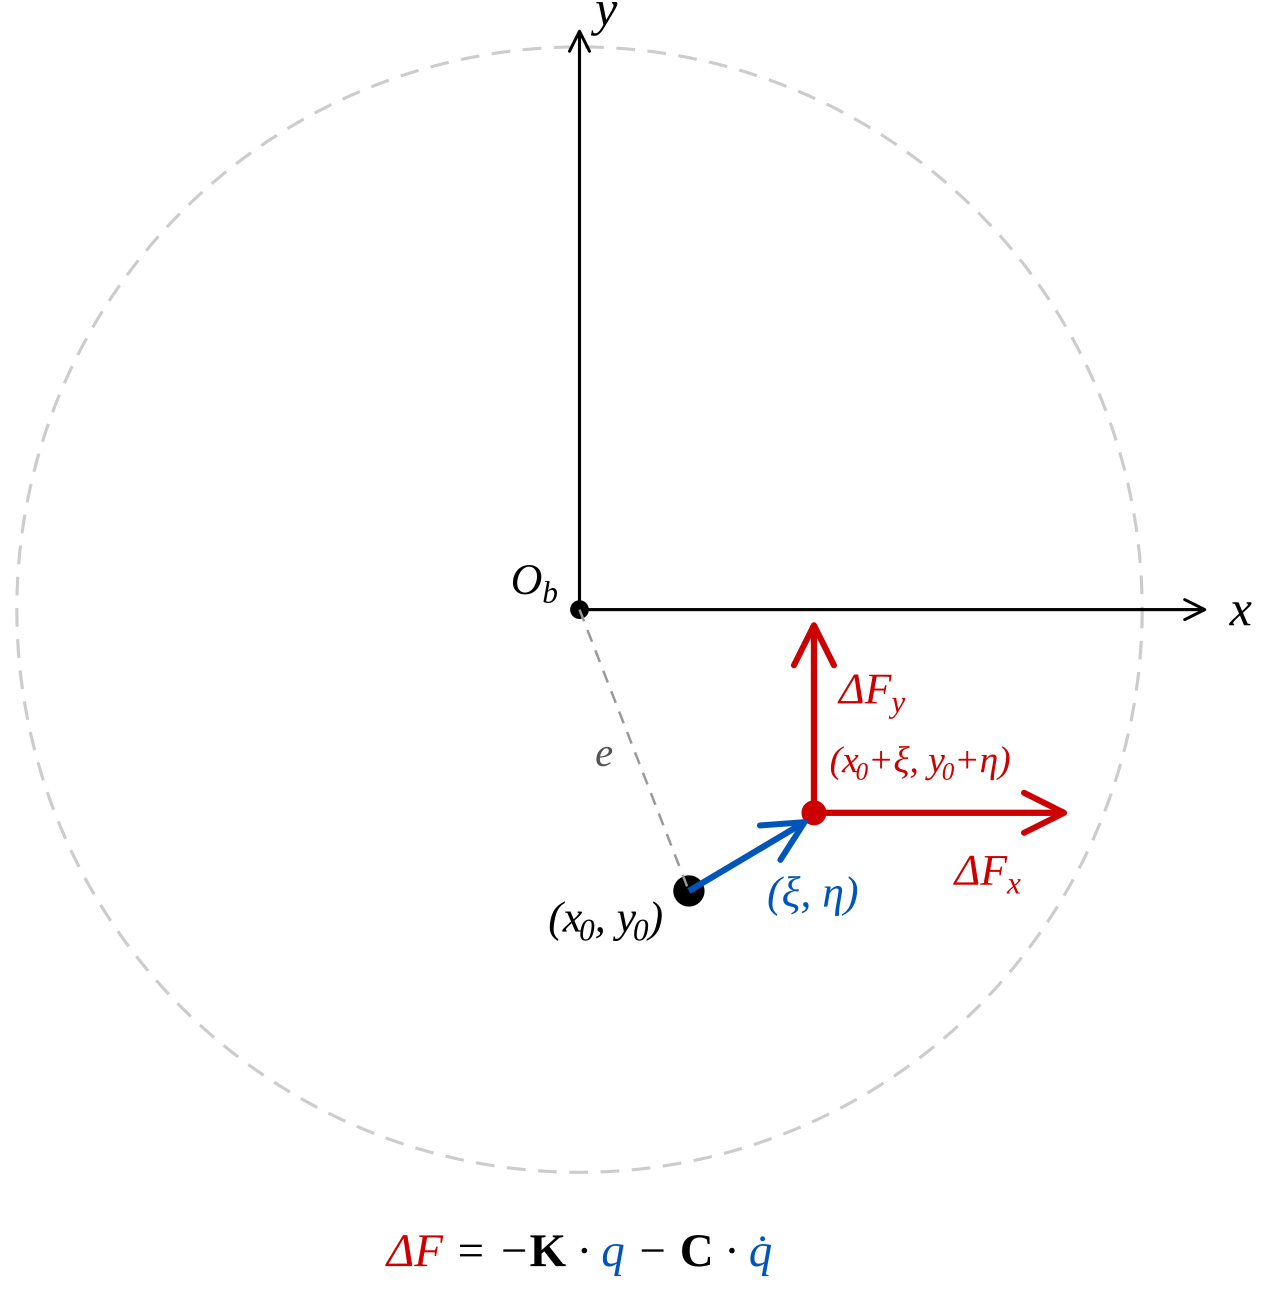
\includegraphics[width=\textwidth,height=0.9\textheight,keepaspectratio]{figures/ch04/fig_4_5.png}
\caption{Линеаризованная модель сил смазочного слоя при малых колебаниях вала}
\label{fig:linearized_forces}
\end{figure}

\FloatBarrier

Линеаризованные коэффициенты жёсткости и~демпфирования
полностью определяются стационарным и~возмущёнными полями
давления; влияние детерминированных микроструктур на~эти
коэффициенты и~устойчивость роторной системы количественно
исследуется в~главе~8.

\textit{Физический смысл прямых и перекрёстных коэффициентов.}
Физический смысл коэффициентов целесообразно пояснить
на примере радиального подшипника. Прямые
жёсткости $K_{xx}$, $K_{yy}$ характеризуют возвращающую силу
при смещении вала вдоль соответствующей оси: $K_{xx} > 0$
означает, что смещение по~$x$ порождает силу, направленную
против смещения (упругоподобное поведение). Прямые
демпфирования $C_{xx}$, $C_{yy}$ определяют диссипативные
силы, противодействующие скорости вала: $C_{xx} > 0$ означает
торможение при движении по~$x$.

Перекрёстные коэффициенты~$K_{xy}$, $K_{yx}$, $C_{xy}$,
$C_{yx}$ описывают связь между двумя направлениями движения.
Для подшипника скольжения перекрёстные жёсткости обычно имеют
противоположные знаки: $K_{xy} > 0$, $K_{yx} < 0$. Это
соответствует циркуляторным силам~-- силам, перпендикулярным
скорости; они не совершают работы в среднем за период,
но могут раскачивать орбиту. Именно наличие циркуляторной пары
$K_{xy} \neq 0$, $K_{yx} \neq 0$ является физическим
механизмом нестабильности типа «вихревая прецессия»
(oil whirl), характерной для подшипников скольжения при
больших скоростях.

\textit{Механизм нестабильности типа вихревой прецессии и~роль текстуры.}
Нестабильность типа oil whirl (вихревая прецессия) возникает, когда циркуляторные силы от~перекрёстных жёсткостей превышают диссипацию от~прямых демпфирований. В~линейной модели~\eqref{eq:rotor_eom} критерий потери устойчивости формулируется через знак~$\mathrm{Re}(\lambda)$, однако физически механизм можно описать следующим образом. При~смещении центра вала по~направлению~$x$ возникает сила~$K_{yx}\,\xi$ в~направлении~$y$ (при~$K_{yx} < 0$ --- это сила, перпендикулярная смещению и~направленная по~вращению). Эта сила раскручивает орбиту вала, постепенно увеличивая её~радиус. Прямое демпфирование~$C_{xx}$, $C_{yy}$ противодействует этому процессу, но~при~достаточно высоких скоростях вращения (и~соответственно высоком давлении смазки) циркуляторная сила превышает диссипацию, и~орбита начинает раскручиваться неограниченно~--- наступает нестабильность.

Детерминированные микроструктуры влияют на~этот баланс через~два канала. С~одной стороны, они изменяют равновесное поле давления~$P_0$ и~тем самым модифицируют все~восемь коэффициентов. С~другой стороны, они изменяют геометрию зазора~$H$, что непосредственно сказывается на~возмущённых полях~$P_\xi$, $P_\eta$, $P_{\dot\xi}$, $P_{\dot\eta}$. Результирующий эффект определяется расположением и~геометрией лунок: текстура во~входной части клина может усиливать прямые жёсткости и~улучшать демпфирование, тогда как~текстура в~зоне убывающего давления оказывает обратное действие~--- это качественно согласуется с~результатами глав~5--7 по~статическому анализу.

\textit{Ограниченность линейной модели.}
Линейная модель~\eqref{eq:rotor_eom} применима только при~малых амплитудах колебаний~$|\xi|, |\eta| \ll c$. При~амплитудах, сопоставимых с~зазором~$c$, нелинейные эффекты становятся существенными: форма орбиты отклоняется от~эллиптической, спектр колебаний обогащается гармониками, а~в~некоторых случаях возникают квазипериодические или хаотические режимы движения. В~этих условиях применение линейных коэффициентов~$K_{ij}$, $C_{ij}$ приводит к~качественно неверным предсказаниям. Полноценный нелинейный анализ требует численного интегрирования уравнений движения с~пересчётом поля давления на~каждом временном шаге, что в~несколько порядков увеличивает вычислительные затраты. Для~целей данной монографии рассматривается только линейная модель; проверка её~применимости выполняется через сравнение максимальных амплитуд с~зазором~$c$ (глава~8).

\textit{Механизм нестабильности типа вихревой прецессии и~роль текстуры.}
Нестабильность типа oil whirl (вихревая прецессия) возникает, когда циркуляторные силы от~перекрёстных жёсткостей превышают диссипацию от~прямых демпфирований. В~линейной модели~\eqref{eq:rotor_eom} критерий потери устойчивости формулируется через знак~$\mathrm{Re}(\lambda)$, однако физически механизм можно описать следующим образом. При~смещении центра вала по~направлению~$x$ возникает сила~$K_{yx}\,\xi$ в~направлении~$y$ (при~$K_{yx} < 0$~--- это сила, перпендикулярная смещению и~направленная по~вращению). Эта сила раскручивает орбиту вала, постепенно увеличивая её~радиус. Прямое демпфирование~$C_{xx}$, $C_{yy}$ противодействует этому процессу, но~при~достаточно высоких скоростях вращения (и~соответственно высоком давлении смазки) циркуляторная сила превышает диссипацию, и~орбита начинает раскручиваться неограниченно~--- наступает нестабильность.

Детерминированные микроструктуры влияют на~этот баланс через~два канала. С~одной стороны, они изменяют равновесное поле давления~$P_0$ и~тем самым модифицируют все~восемь коэффициентов. С~другой стороны, они изменяют геометрию зазора~$H$, что непосредственно сказывается на~возмущённых полях~$P_\xi$, $P_\eta$, $P_{\dot\xi}$, $P_{\dot\eta}$. Результирующий эффект определяется расположением и~геометрией лунок: текстура во~входной части клина может усиливать прямые жёсткости и~улучшать демпфирование, тогда как~текстура в~зоне убывающего давления оказывает обратное действие~--- это качественно согласуется с~результатами глав~5--7 по~статическому анализу.

\textit{Ограниченность линейной модели.}
Линейная модель~\eqref{eq:rotor_eom} применима только при~малых амплитудах колебаний~$|\xi|, |\eta| \ll c$. При~амплитудах, сопоставимых с~зазором~$c$, нелинейные эффекты становятся существенными: форма орбиты отклоняется от~эллиптической, спектр колебаний обогащается гармониками, а~в~некоторых случаях возникают квазипериодические или хаотические режимы движения. В~этих условиях применение линейных коэффициентов~$K_{ij}$, $C_{ij}$ приводит к~качественно неверным предсказаниям. Полноценный нелинейный анализ требует численного интегрирования уравнений движения с~пересчётом поля давления на~каждом временном шаге, что в~несколько порядков увеличивает вычислительные затраты. Для~целей данной монографии рассматривается только линейная модель; проверка её~применимости выполняется через сравнение максимальных амплитуд с~зазором~$c$ (глава~8).

\textit{Связь с главой~8 и метод численного вычисления
коэффициентов.}
Аналитическое вычисление коэффициентов~$K_{ij}$, $C_{ij}$
через интегралы~\eqref{eq:K_integrals} требует решения
четырёх вспомогательных линеаризованных уравнений Рейнольдса.
Альтернативный численный подход, используемый в главе~8,
основан на методе центральных конечных разностей:
коэффициент $K_{xx}$ вычисляется как
$K_{xx} \approx -[F_x(x_0 + \Delta x) -
F_x(x_0 - \Delta x)]/(2\Delta x)$, где $F_x$ получается
прямым решением стационарного уравнения Рейнольдса при
возмущённом зазоре. Аналогично для коэффициентов демпфирования
решается динамическое уравнение Рейнольдса с ненулевой
скоростью возмущения~$\dot{x}$ или~$\dot{y}$. Точность
такого подхода определяется величиной шага конечных
разностей~$\Delta x$, $\Delta v$: при слишком большом шаге
нарушается линейное приближение, при слишком малом~-- результат
искажается численным шумом; оптимальный диапазон обсуждается
в разделе~8.4.


\FloatBarrier
\section*{Контрольные вопросы}
\phantomsection\addcontentsline{toc}{section}{Контрольные вопросы}

\begin{enumerate}
\item Что~такое кавитация в~контексте смазочного слоя?
\item Что~такое число подшипника~$\Lambda$ и~как оно~связано с~нелинейностью?
\item Как~учитывается изменение плотности смазки?
\item Какие термовязкостные эффекты влияют на~работу подшипника?
\item Как~зависит вязкость масла от~температуры?
\item Что~такое модель Патира--Ченга для~учёта шероховатости?
\item Какое влияние оказывает шероховатость на~нагрузочную способность?
\item В~чём отличие стохастической и~детерминированной моделей шероховатости?
\item Какие уровни учёта температуры существуют при~моделировании смазочного слоя?
\item Что~такое число смазочного слоя~$\lambda_r$ и~как оно~определяет режим трения?
\end{enumerate}
